\section{参数与处理顺序的影响}
\label{sec:parameters}

\subsection{时间和距离阈值怎样改变切分}
初始设置能运行，并不意味着它适合所有记录。首先只改变一项参数，其余保持参考值，再检查切分、过滤和后续输出的变化。表\ref{tab:grid}列出测试范围，另对时间与距离、点数与长度分别作$5\times5$联合实验。去除重复设置后，初轮开发共比较59个完整配置，而非穷举六参数的所有组合。

\begin{table}[htbp]\centering\small
\caption{初轮开发的离散参数范围}\label{tab:grid}
\begin{tabularx}{\linewidth}{@{}L{42mm}Y@{}}\toprule
参数 & 实际比较值\\\midrule
时间差 / 秒 & 15，20，30，45，60\\
距离 / 工作米 & 95，200，400，600，800\\
最少点数 & 2，3，5，7，10\\
最短累计长度 / 工作米 & 0，32.5，65，97.5，130\\
方向差 / 度 & 15，25，35，45，60\\
DP容差 / 工作米 & 0，0.5，1，2，5，10，20\\\bottomrule
\end{tabularx}
\end{table}

时间阈值过小，可能把正常的较疏采样切成许多短段，再被过滤。表\ref{tab:time-distance}中，15秒使片段数由参考的344增至2,418，共同覆盖由8,408降至4,595点。这个结果说明，更多分段并不自动代表更准确地找到了行程边界。反过来，放宽阈值虽然可能少切几段，却需要检查是否重新跨越共同参考中的断点。

\begin{table}[htbp]\centering\small
\caption{时间、距离单因素比较。每行均为120条记录、11,777个原始点，其余参数不变}\label{tab:time-distance}
\begin{tabular}{@{}lrrrrr@{}}\toprule
变化参数 & 取值 & 片段数 & 共同覆盖点 & 无输出记录 & 跨断点边\\\midrule
时间差 / 秒 & 15 & 2,418 & 4,595 & 45 & 0 \\
时间差 / 秒 & 20 & 720 & 7,608 & 33 & 0 \\
时间差 / 秒 & 30 & 344 & 8,408 & 33 & 0 \\
时间差 / 秒 & 45 & 314 & 8,353 & 32 & 17 \\
时间差 / 秒 & 60 & 308 & 8,376 & 31 & 19 \\
\midrule
距离 / 工作米 & 95 & 2,883 & 5,014 & 42 & 0 \\
距离 / 工作米 & 200 & 1,220 & 7,397 & 35 & 0 \\
距离 / 工作米 & 400 & 344 & 8,408 & 33 & 0 \\
距离 / 工作米 & 600 & 218 & 8,253 & 33 & 121 \\
距离 / 工作米 & 800 & 206 & 8,225 & 33 & 130 \\

\bottomrule
\end{tabular}
\tabnote{跨断点边按预先固定的原始30秒／400工作米窗口判断。该条件用于共同比较，不把它解释成真实出行边界标签。时间与距离均取参考值的那一行，在两个单因素组中相同。}
\end{table}

这些实验将时间差30秒、距离400工作米保留为后续共同起点。理由不是默认值具有优先权，而是所测替代设置没有在共同条件下形成可统一采用的改善；95工作米示例也未因此被当作必须适用于本数据的界限。

\subsection{哪些短段过滤条件造成信息丢失}
片段短或点少，并不等于所有观测都没有表达价值。为区分两道过滤条件，固定切分、方向和简化参数，只改变最少点数与最短长度。图\ref{fig:surface}展示全部25个组合的共同覆盖率。

\begin{figure}[H]\centering
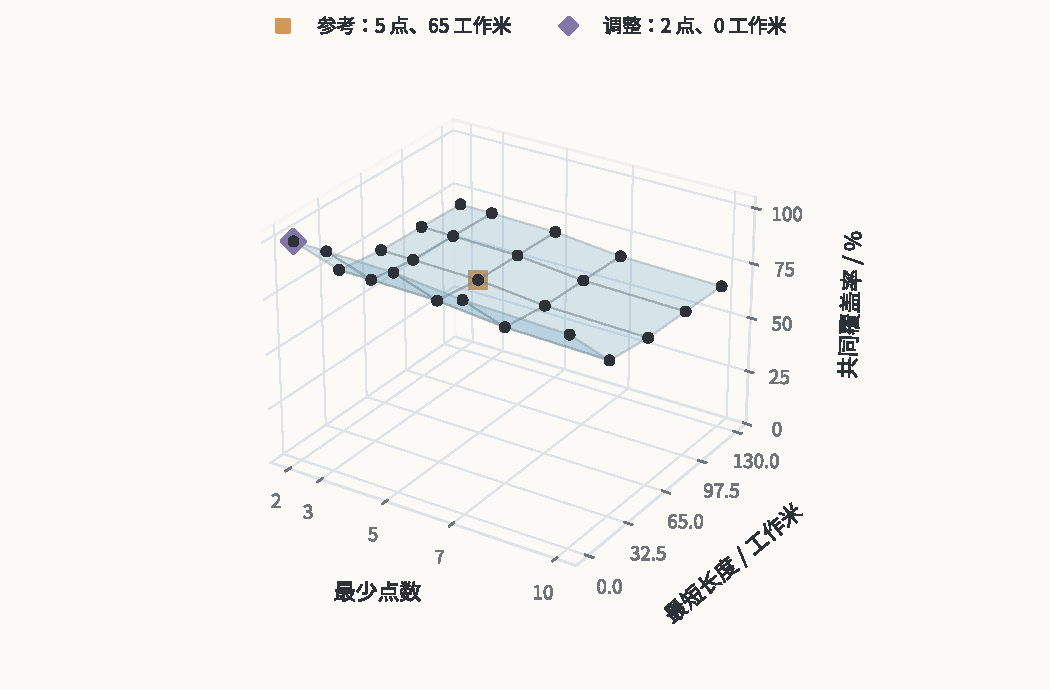
\includegraphics[width=.99\linewidth]{figures/filter_parameter_surface.pdf}
\caption{过滤条件的三维响应网格。分母均为11,777个原始点，黑点为已测试设置；网格面只连接相邻观测，不表示未测位置也有实验结果。杏色方点为参考设置，紫色菱形为后续过滤调整设置。}\label{fig:surface}
\end{figure}

较高的长度门槛会丢弃一批原本包含多个点的片段。取消正长度下限、并将最少点数降到2后，更多原始范围进入后续处理。这里的高度只表示共同覆盖率，不能单凭曲面最高的位置认定真实清洗质量最好；候选还需满足几何、断点和记录保留条件。

在另外120条阶段评估记录中，这一过滤调整全部通过登记保护，53条共同覆盖严格增加。覆盖从8,805增至12,162点，无输出记录从32降到0；显式保留点从2,748增至2,939。新增表达范围远多于新增存储点，说明后续简化仍在发挥作用。

这时仍不能判断两项调整是否都必要，也不知道增加其他规则是否会更好。第\ref{sec:selection}章把点数和长度门槛拆开核验，再检查有依据的组合，而不直接把所有改动叠入最终方案。

\clearpage
\subsection{方向阈值与简化容差的取舍}
放宽方向差阈值，会减少满足双侧删除条件的点。但保留更多点是否改善完整轨迹，还取决于其位置和后续简化，不能由删除数量直接判断。

\begin{figure}[H]\centering
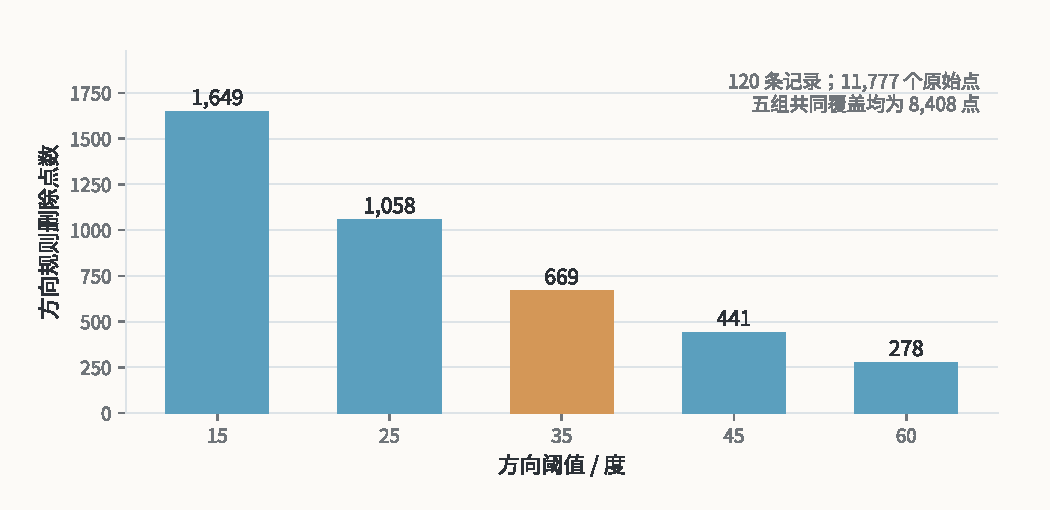
\includegraphics[width=.89\linewidth]{figures/direction_parameter.pdf}
\caption{方向阈值对删除点数的影响。相同开发范围内仅改变方向阈值，参考35度用杏色标出。阈值较宽时删除较少，但五组共同覆盖均为8,408点；这不是噪声准确率曲线。}\label{fig:direction}
\end{figure}

15、35、60度分别删除1,649、669、278点。差异体现了规则的敏感性，但共同覆盖不变，并不意味着几何变化也相同。初轮没有找到能统一替换35度的方向阈值，因而先保留参考，后续只在有明确原始诊断依据时检查条件规则。

DP的取舍更直接：较紧容差通常需要更多保留点，较宽容差可能更精简，但允许更大偏差。图\ref{fig:dp}在同一完整P输入上比较各容差，不将方向删除带来的变化混入压缩收益。

\begin{figure}[H]\centering
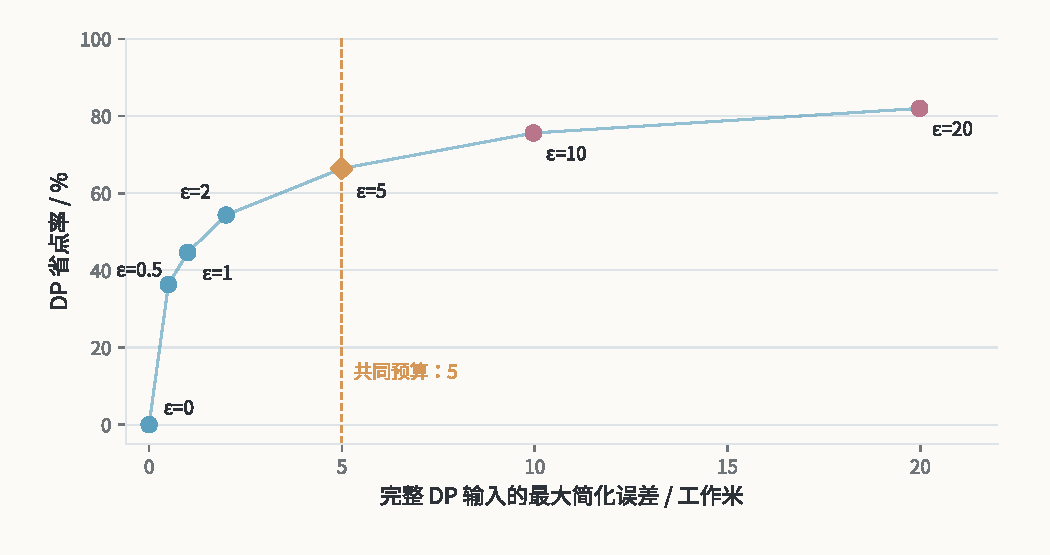
\includegraphics[width=.89\linewidth]{figures/dp_error_saving.pdf}
\caption{相同上游输入上的DP误差与省点率。点旁标记为容差，连线仅连接已测设置。杏色虚线为共同5工作米预算；0是不简化参照，实际超预算的设置用玫瑰色标出。}\label{fig:dp}
\end{figure}

缩小容差带来较低即时误差，却未在共同预算下产生额外省点收益；10、20工作米可展示更宽容差的影响，但实际超出5时不满足最终方案的误差要求。初轮方向与DP单项因此都保留参考设置，而不是为使候选不同而强选新值。

在所测单因素相邻取值之间，也未出现阶段索引、覆盖与各阶段点数全部相同的精确稳定区间。结论仅限这些离散测试，不能由几条相近的平均值推出连续参数范围都稳定。

\subsection{三种操作能否交换顺序}
每一步都改变下一步看到的输入，所以顺序本身也是需要验证的变量。表\ref{tab:orders}比较六种排列。S均包含切分及紧随其后的过滤；D、P在前时没有暗中添加相同的预分段，所有邻接特征在实际变化后重新计算。

\begin{table}[htbp]\centering\small
\caption{六种顺序在120条开发记录上的检查结果}\label{tab:orders}
\begin{tabularx}{\linewidth}{@{}lrrrrY@{}}\toprule
顺序 & 安全失败记录 & 跨断点边 & D跨断点窗口 & P删触发点 & 判断\\\midrule
S-D-P & 0 & 0 & 0 & 0 & 保留参考\\
S-P-D & 0 & 0 & 0 & 0 & 有权衡\\
D-S-P & 46 & 1 & 612 & 1 & 未通过\\
D-P-S & 87 & 1 & 612 & 188 & 未通过\\
P-S-D & 87 & 0 & 0 & 193 & 未通过\\
P-D-S & 87 & 1 & 453 & 193 & 未通过\\\bottomrule
\end{tabularx}
\tabnote{“安全失败”按记录计，后三列按事件计，不能相加。“P删触发点”表示简化删除了原始断点判定所需的观测。表中安全是本实验的共同约束，不是交通安全判断。}
\end{table}

D在S之前时，方向窗口可能跨越本来需要断开的空档。P在S之前时，则可能先移除触发断点的点，令后面的切分看不到原始信息。四种出现实际失败的顺序未继续作为统一改进候选；这类约束拒绝是实验结果，不是需要把方法修到通过的代码错误。

S-P-D在开发及阶段评估中没有出现上述安全失败，但P之后的D会再次改写几何。阶段评估中，S-D-P的共同原始最大偏差约136.118工作米，S-P-D约377.727工作米，而后者P即时误差仍约4.993工作米。局部容差因此不能替代最终几何检查。

这些对照说明三步不能无条件交换，并支持在本次定义、数据与比较规则下保留S-D-P；它们并不意味着所有轨迹任务永远只能使用这一顺序。
